\documentclass[10pt,a4paper, onecolumn, conference]{IEEEtran}
\author{Adam Lee}
\title{Multiple Linear Regression}
\date{November 2020}
\usepackage{amsthm}
\usepackage{pgfplots}
\usepackage{graphicx}
\usepackage{float}
\usepackage{amsmath}
\usepackage{amsfonts}
\usepackage{amssymb}
\usepackage{verbatim}
\usepackage{amsbsy}
\usepackage{algorithm}
\usepackage{algorithmic}
\usepackage[T1]{fontenc}
\usepackage[utf8]{inputenc}
\usepackage{hyperref}
\usepackage{cleveref}
\usepackage{placeins}
\usepackage{subcaption}
\usepackage{tablefootnote}
\DeclareMathOperator{\var}{var}
\renewcommand{\tabcolsep}{18pt}
\newtheoremstyle{own}%
    {5pt}% Space above
    {5pt}% Space below
    {}% Body font
    {}% Indent amount
    {\color{black}\bfseries}% Theorem head font
    {:}% Punctuation after theorem head
    {5pt}% Space after theorem head
    {}% Theorem head spec
\theoremstyle{own}
\newtheorem{example}{Example}
\theoremstyle{definition}
\newtheorem{definition}{Definition}
\theoremstyle{plain}
\newtheorem{thm}{Theorem}
\begin{document}
\maketitle
\pagebreak
\section{Introduction}
Our definition of linearity yields a significant amount of flexibility for our regression models. We can extend our definition for simple linear regression to form a regression model with multiple regressors each of which does not itself need to be linear but instead is accompanied by a coefficient which is linearly related to $y$. That is we can fit a model
\begin{equation} \label{eq1}
y = \beta_0 + \beta_1 \phi_1(x) + \cdots + \beta_k \phi_k(x) + \varepsilon,
\end{equation}
where $y$ is our response variable and $\phi_i$ for $i = 1, \ldots, k$ are our basis functions evaluated at our regressor $x$. It must be noted the term linear is used here since \cref{eq1} is a linear function of the unknown parameters $\beta_i$. This means we can choose our regressor terms freely. More complex models may allow for a polynomial fit such as in~\cref{ex1}.
\begin{example} \label{ex1}
Consider the polynomial model
\begin{equation}
y = \beta_0 + \beta_1 x + \beta_2 x^2 + \varepsilon.
\end{equation}
If we let $\phi_i(x) := x^i$ then this model takes the form
\begin{equation}
y = \beta_0 + \beta_1 \phi_1(x) + \beta_2 \phi_2(x) + \varepsilon,
\end{equation}
and is a linear regression model with three unknown regression coefficients and two regressors. It is still linear in our coefficients $\beta_i$, however, allows for a much more flexible model. The inclusion of more regressors than our simple model presents opportunities for linear regression in higher dimensions [\ref{fig1}], while the consideration of basis functions $\phi$ allows us to consider relationships between the response variable $y$ and the regressors which are not themselves linear.
\end{example}

We can extend our definition of a multiple linear regression model further to include interaction terms. For example, consider the model
\begin{equation}
y = \beta_0 + \beta_1 x_1 + \beta_2 x_2 + \beta_{12} x_1 x_2,
\end{equation}
which is still linear in the parameters $\beta_i$.

\section{Multiple Linear Regression}
Let us focus on the generic case with model
\begin{equation}
y = \beta_0 + \beta_1 x_1 + \cdots + \beta_k x_k + \varepsilon.
\end{equation}

Here our regressor $\mathbf{x} = \left[ x_1, x_2, \ldots, x_k \right]^{\text{T}}$ is a vector and our basis functions $\phi_i(\mathbf{x}) = x_i,~~ i = 1, \ldots, k$ simply return each component of the regressor. This model describes a $k$ dimension hyperplane, as opposed to the regression line we constructed for the simple case. The parameters $\beta_i$ are our regression coefficients and in practice these, as well as the variance of the error $\epsilon$, are unknown. The particular parameter $\beta_j$ represents the expected change in $y$ per unit change in $x_j$ under the assumption that all other regressors $x_i,~( i \neq j )$ are constant. Figure \ref{fig1} provides graphic representation of a two-regressor, non-interacting model.
\vspace{2mm}
\hrule
\begin{example}
Consider a model where our expected error is zero
\begin{equation} \label{eq2}
E(y) = 10 + 15x_1 + 4x_2.
\end{equation}
We can examine the hyperplane of dimension 2\footnote{A plane of dimension $d$ embedded into a space of dimension $d+1$ is a hyperplane of dimension $d$.} this model describes [\ref{fig1}].
\begin{figure}[H]
\centering
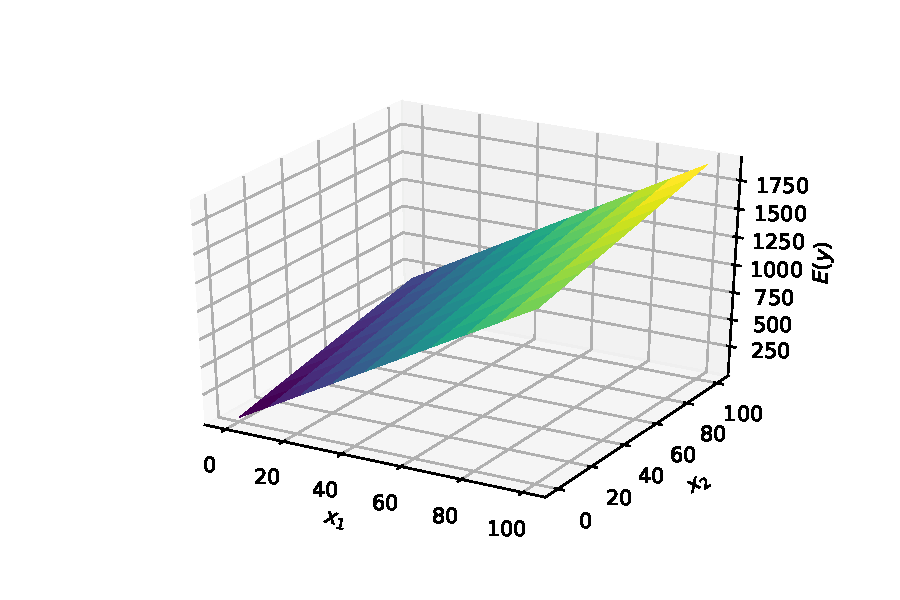
\includegraphics[width = 0.5\textwidth]{f4}
\caption{Hyperplane plot for \cref{eq2}}
\label{fig1}
\end{figure}
\end{example}
\hrule
\vspace{2mm}

Let us assume we have a data-set $\varkappa = \{y_i, x_{i1}, \ldots, x_{ik} \}_{i=0}^n$ where $k > n$. Here, $y_i$ denotes the $i$-th observed response and $x_{ij}$ denotes the observed value $x_i$ for regressor $x_j$. Then, we have a system of model equations
\begin{equation}
y_i = \beta_0 + \beta_1 x_{i1} + \beta_2 x_{i2} + \cdots + \beta_k x_{ik} ~~ i = 0, \ldots, n.
\end{equation}
We can then assume matrix notation for the entire set such that
\begin{equation}
\mathbf{y} = X \boldsymbol\beta + \boldsymbol\varepsilon.
\end{equation}
where
\begin{equation}
\mathbf{y} = \left( \begin{matrix} y_0 \\ y_1 \\ \vdots \\ y_n \end{matrix} \right),
\end{equation}
\begin{equation}
X = \left( \begin{matrix}
1 & x_{01} & \cdots & x_{0k} \\
1 & x_{11} & \cdots & x_{1k} \\
\vdots & \vdots & \ddots & \vdots \\
1 & x_{n1} & \cdots & x_{nk} 
\end{matrix} \right),
\end{equation}
\begin{equation}
\boldsymbol\beta = \left( \begin{matrix} \beta_0 \\ \beta_1 \\ \vdots \\ \beta_k \end{matrix} \right),
\end{equation}
and
\begin{equation}
\boldsymbol\varepsilon = \left( \begin{matrix} \varepsilon_0 \\ \varepsilon_1 \\ \vdots \\ \varepsilon_n \end{matrix} \right).
\end{equation}
The task then becomes fitting this linear model such that the coefficients $\boldsymbol\beta$ minimize the error term $\boldsymbol\varepsilon = \mathbf{y} - X \boldsymbol\beta$. A common method for determining these parameters is the method of least-squares, which we have already come across for the simple linear regression case. The same principles can be extended to multiple linear regression.
\section{Method of Least-Squares}
Let us define the multivariate least-squares criterion function
\begin{align} \nonumber
\mathbf{E}(\boldsymbol\beta) := \sum_{i = 0}^n \varepsilon_i^2 & = \boldsymbol\varepsilon^{\text{T}} \boldsymbol\varepsilon = (\mathbf{y} - X \boldsymbol\beta)^{\text{T}} (\mathbf{y} - X \boldsymbol\beta) \\
& = \mathbf{y}^{\text{T}}\mathbf{y} - 2\boldsymbol\beta^{\text{T}}X^{\text{T}}\mathbf{y} + \boldsymbol\beta^{\text{T}}X^{\text{T}} X\boldsymbol\beta.
\end{align}
Then, we look for $\hat{\boldsymbol\beta} \in \mathbb{R}^{k+1}$ such that
\begin{equation}
\arg \min \mathbf{E} (\boldsymbol\beta) = \hat{\boldsymbol\beta}.
\end{equation}
To do so we must have
\begin{equation}
\frac{\partial \mathbf{E}}{\partial \boldsymbol\beta} \Big|_{\hat{\boldsymbol\beta}} = -2X^{\text{T}}\mathbf{y} + 2 X^{\text{T}} X \hat{\boldsymbol\beta} =  0,
\end{equation}
which we can simplify to
\begin{equation}
X^{\text{T}} X \hat{\boldsymbol\beta} = X^{\text{T}}\mathbf{y}.
\end{equation}
Then, provided the inverse matrix $(X^{\text{T}} X)^{-1}$ exists, our solution is
\begin{equation}
\hat{\boldsymbol\beta} = (X^{\text{T}} X)^{-1} X^{\text{T}}\mathbf{y}.
\end{equation}
Let us examine the matrix $X^{\text{T}} X$ in detail. By \cref{posdef}, $X^{\text{T}} X$ is a positive-definite matrix of the form, setting $p = n+1, q = k+1$
\begin{equation*} \arraycolsep=1.4pt\def\arraystretch{2.2}
\left[ \begin{array}{ccccc} p^2 & \sum_{i = 0}^n x_{i1} & \sum_{i = 0}^n x_{i2} & \cdots & \sum_{i = 0}^n x_{ik} \\
             \sum_{i = 0}^n x_{i1} & \sum_{i = 0}^n x_{i1}^2 & \sum_{i = 0}^n x_{i1}x_{i2} & \cdots & \sum_{i = 0}^n x_{i1}x_{ik} \\
             \sum_{i = 0}^n x_{i2} & \vdots & \ddots & & \vdots\\
             \vdots				   & \vdots &  & \ddots & \vdots \\
             \sum_{i = 0}^n x_{ik} & \sum_{i = 0}^n x_{i1}x_{ik}  & \cdots & \cdots & \sum_{i = 0}^n x_{ik}^2

\end{array} \right]
\end{equation*}
The computational complexity of matrix inversion is of order $\mathbf{O}(n^3)$ for an $n\times n$ matrix. However, the matrix $X^{\text{T}}X$ is positive-definite [\ref{ap:2}] and therefore we can compute its inverse using Cholesky arithmetic. This process has complexity of order $\mathbf{O}(\frac{1}{2} n^3)$. We can then utilise our parameters on some set of test points, say $\mathbf{x}^{*}$ then
\begin{equation}
\hat{\mathbf{y}} = \hat{X} \hat{\boldsymbol\beta} = \hat{X} (X^{\text{T}} X)^{-1} X^{\text{T}}\mathbf{y} = H\textbf{y},
\end{equation}
where $\hat{X}$ is the corresponding $X$ for the test points $\mathsf{x}^{*}$. We call the matrix $H$ the hat matrix of our model.
\section{Basis Functions}
Our generic example considers the construction of a $k$ dimension hyperplane, which we can visualise in up to two dimensions as in \cref{fig1}. Let us instead consider examples more akin to~\cref{ex1} where our model takes the form
\begin{equation}
y = \sum_{i = 0}^{k} \beta_i \phi_i(x) + \epsilon,
\end{equation}
where $\beta_i$ are our unknown parameters, and $\phi_i$ are basis functions. Then we can assume matrix notation for our data set $\varkappa$
\begin{equation}
\mathbf{y} = X \boldsymbol\beta + \boldsymbol\varepsilon.
\end{equation}
where
\begin{equation}
\mathbf{y} = \left( \begin{matrix} y_0 \\ y_1 \\ \vdots \\ y_n \end{matrix} \right),
\end{equation}
\begin{equation}
X = \left( \begin{matrix}
\phi_0(x_0) & \phi_1(x_0) & \cdots & \phi_k(x_0) \\
\phi_0(x_1) & \phi_1(x_1) & \cdots & \phi_k(x_1) \\
\vdots & \vdots & \ddots & \vdots \\
\phi_0(x_n) & \phi_1(x_n) & \cdots & \phi_k(x_n) \\
\end{matrix} \right),
\end{equation}
\begin{equation}
\boldsymbol\beta = \left( \begin{matrix} \beta_0 \\ \beta_1 \\ \vdots \\ \beta_k \end{matrix} \right),
\end{equation}
and
\begin{equation}
\boldsymbol\varepsilon = \left( \begin{matrix} \varepsilon_0 \\ \varepsilon_1 \\ \vdots \\ \varepsilon_n \end{matrix} \right).
\end{equation}
Then our solution for our parameters is nothing else than
\begin{equation}
\hat{\boldsymbol\beta} = (X^{\text{T}} X)^{-1} X^{\text{T}}\mathbf{y}.
\end{equation}
\subsection{Basis Function Examples}
Our basis functions can assume any form such that each function $\phi_i$ is real-valued and scalar. Two popular basis functions are polynomial and Gaussian radial basis functions.
\begin{example}[Polynomial Regression]
Polynomial regression uses basis functions
\begin{equation}
\boldsymbol\phi = \left[ \begin{matrix} 1 & x & x^2 & \cdots & x^k  \end{matrix} \right]^{\text{T}},
\end{equation}
then our matrix $X$ would become
\begin{equation}
X = \left( \begin{matrix}
1 & x_0 & \cdots & x_0^k \\
1 & x_1 & \cdots & x_1^k \\
\vdots & \vdots & \ddots & \vdots \\
1 & x_n & \cdots & x_n^k \\
\end{matrix} \right).
\end{equation}
Restricting our basis functions to $\boldsymbol\phi = \left[ \begin{matrix} 1 & x \end{matrix} \right]^{\text{T}}$ gives us simple linear regression. In \cref{fig2}, we generated 100 data-points $y_i, i = 1, \ldots, 100$ of the form
\begin{equation}
y_i = f(x_i) + \varepsilon, ~~~~ f(x) = 2 + x + x^2 - \frac{1}{100} x^3, ~~~~ \varepsilon \thicksim \mathcal{N} \left( 0, 1000 \right),
\end{equation}
which are plotted in blue. The red curve is our regression line computed using MLE fitting a model of the form
\begin{equation}
y = \beta_0 + \beta_1 \phi_1(x) + \beta_2 \phi_2(x) + \beta_3 \phi_3(x), ~~ \phi_i(x) = x^i,
\end{equation}
to our observations.
\begin{figure}[H]
\centering
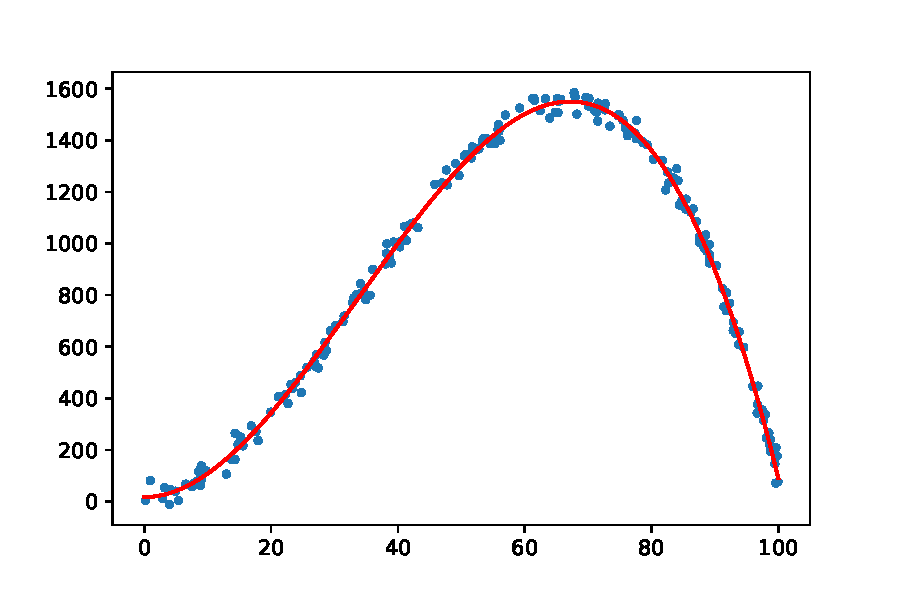
\includegraphics[width = 0.8\textwidth]{polyBF_example}
\caption{Example of polynomial regression}
\label{fig2}
\end{figure}
\hrule
\vspace{2mm}
\end{example}
\begin{example}[Gaussian Radial Basis Functions]
Let us now consider Gaussian radial basis functions
\begin{equation}
\phi_i(x) = e^{-\lambda^{2} ( x - \mu_i ) ^{2} }
\end{equation}
where $\lambda$ is some coefficient representing the variance of our basis functions and $\boldsymbol\mu = \left[ \begin{matrix} \mu_1 & \cdots & \mu_n \end{matrix} \right]^{\text{T}}$ are centres for each Gaussian. Then our predictive function becomes a linear combination of weighted Gaussians where our parameters $\lambda$ and $\mu_i$ determine the smoothness of this function on our test interval. There arises the problem of under or over-fitting our data should we include poor hyper-parameters or attempt to fit too many/few Gaussians to our data.

Consider \cref{fig3}, here our data was generated in a similar fashion to \cref{fig2}. Our generating function in this case was
\begin{equation}
y_i = f(x_i) + \varepsilon, ~~~~ f(x) = x \sin(0.5x), ~~~~ \varepsilon \thicksim \mathcal{N} \left( 0, 1 \right).
\end{equation}
Our basis functions were of the form
\begin{equation}
\phi_i = e^{-0.5 ( x - i ) ^{2} },~~ i = -10, \ldots, 10,
\end{equation}
that is, we fit a RBF centred at each integer within the domain of our data.
\begin{figure}[H]
\centering
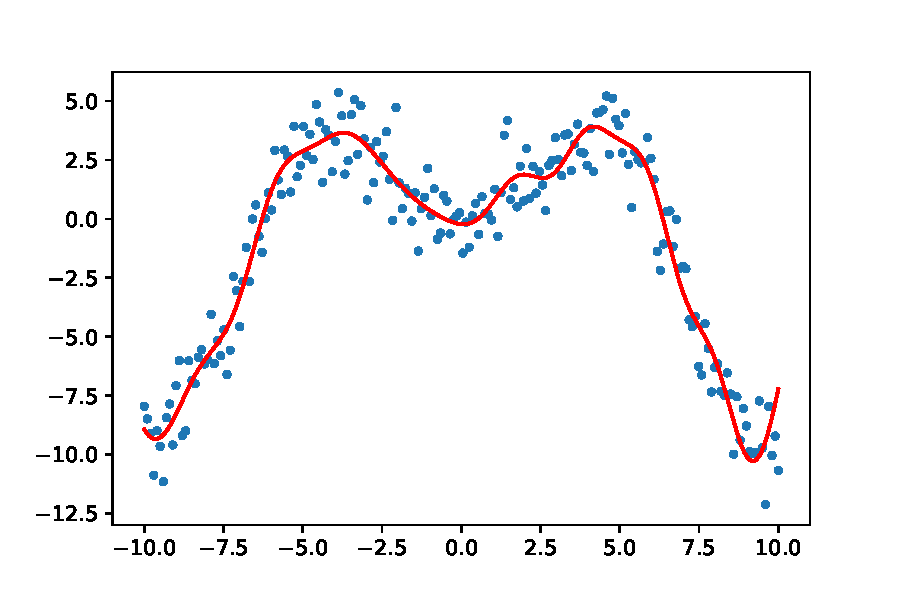
\includegraphics[width = 0.8\textwidth]{f5}
\caption{Example of linear regression using Gaussian radial basis functions}
\label{fig3}
\end{figure}
\end{example}












\pagebreak
\appendix
\section{Linear Algebra Proofs}
\begin{thm} \label{posdef}
For any real, invertible matrix $A \in \mathbb{R}^{n \times n}$, the product matrix $A^{\text{T}}A$ is positive definite i.e
\begin{equation}
\mathbf{z}^{\text{T}} A^{\text{T}}A \mathbf{z} > 0 ~ \forall ~ \mathbf{z} \in \mathbb{R}^{n}
\end{equation}
\end{thm}
\begin{proof}
\begin{align} \nonumber
\mathbf{z}^{\text{T}} A^{\text{T}}A \mathbf{z} & = (A \mathbf{z})^{\text{T}} (A \mathbf{z}) \\
& = || Az ||^2 > 0.
\end{align}
\end{proof}
\begin{thm} \label{ap:2}
For a positive-definite matrix $A$, there exists a lower-triangular matrix $U$ such that
\begin{equation}
A^{-1} = U U^{T}
\end{equation}
\end{thm}
\begin{proof}
For positive-definite matrix $A$, we have a Cholesky decomposition such that
\begin{equation}
A = L L^{\text{T}},
\end{equation}
then we have
\begin{equation}
A A^{-1} = L L^{\text{T}} A^{-1} = I,
\end{equation}
that is
\begin{equation}
A^{-1} = ( L^{\text{T}} )^{-1} L^{-1}.
\end{equation}
Since $L$ is lower triangular, if we write $( L^{\text{T}} )^{-1} = U$ then we have
\begin{equation}
A^{-1} = U U^{\text{T}},
\end{equation}
which is a positive-definite symmetric matrix such that we need only compute the upper-triangular elements of $U U^{\text{T}}$ in order to know all elements of $A^{-1}$.
\end{proof}













 
\end{document}
